\documentclass[9pt]{beamer}
\usepackage{circuitikz}
\urlstyle{same}

\title{Non-Linear Dynamics (NLD)}
\author{Eric Du}
\institute{University of California, Berkeley}
\date{\today}

%\mode<presentation>
\usetheme{Goettingen}
\ctikzset{diodes/scale=0.6}
\ctikzset{capacitors/scale=0.6}
\ctikzset{sources/scale=0.6}

\AtBeginSection[]
{
  \begin{frame}
    \frametitle{Table of Contents}
    \tableofcontents[currentsection]
  \end{frame}
}

\begin{document}
	
\frame{\titlepage}

\begin{frame}
	\frametitle{Outline}
	\tableofcontents
\end{frame}

\section{What is NLD?}
\begin{frame}
	\frametitle{Dynamics}
	\begin{itemize}
		\item The study of how a system evolves through time. 
			\pause 
		\item \textit{How do I model the motion of a ball when I throw it up?}
			\pause 
		\item \textit{What happens if I place a pendulum at an angle 
			\( \theta \) and let go?}
			\pause 
		\item \textit{What happens to the sequence \( \{x_n\} \) if I start at 
				\( x_0 \) and iterate with the rule \( x_1 = f(x_0) \) 
			for some \( f \) of my choosing?} 
			\pause 
		\item One thing we care about is whether the system is \textit{linear}
	\end{itemize}
\end{frame}

\begin{frame}
	\frametitle{Nonlinearity}
	\begin{itemize}
		\item When a derivative in the differential equation (equation of motion) has a 
			square term or higher, or has a cross term involving two derivatives.  
			\begin{itemize}
				\item More formally, the differential equation is linear if it can be
					expressed as a linear polynomial:
					\[
						a_0(x)y + a_1(x) y' + \dots + a_n(x) y^{(n)} = b(x) 
					\]
					\( a_0(x), \dots, a_{n}(x) \) and \( b(x) \) need not be linear. 
			\end{itemize}
		\item As for the examples in the previous slide:
			\begin{itemize}
				\item Ball: \( y(t) = \dot y(0) t - \frac{1}{2}\ddot y t^2 \pause \implies \text{Linear.} \)  
					\pause 
				\item Pendulum: \( \ddot \theta - \frac{g}{L} \sin \theta 
					= 0 \pause \implies \text{Nonlinear.}\)
					\pause
				\item \( \{x_n\} \) sequence: \pause depends on \( f \)!
			\end{itemize}
	\end{itemize}
\end{frame}


\begin{frame}
	\frametitle{What is Chaos?}

	\begin{itemize}
		\item \textbf{Aperiodic:} Over long time, the behavior appears 
			random and does not settle into a periodic state, where the same state is
			visited infinitely many times. 
		\item \textbf{Deterministic:} Given a specific set of initial
			conditions, we can predict the evolution of the system 
			through time. 
		\item \textbf{Sensitive Dependence on Initial Conditions:} 
			Trajectories which start off with an infinitesimal deviation 
			diverge exponentially quickly (we will come back to this). 
	\end{itemize}
\end{frame}

\section{The Logistic Map}

\subsection{Recursive Sequences}
\begin{frame}
	\frametitle{Recursive Sequences}
	\begin{itemize}
		\item Characterized by a recursive relation \( x_{n+1} = f(x_{n-1}, 
			x_{n - 2}, \dots,  x_0) \). 
		\item e.g. The Fibonacci sequence: \( f_n = f_{n - 1} + f_{n - 2} \)
		\item Our recursive equation of interest: \( x_{n+1} = 
			f(x_n) = rx_n(1 - x_n) \), 
			sometimes called the logistic equation.
		\item We control the value of \( r \), and are interested in how 
			the sequence \( x_n \) evolves through successive 
			iterations. 
		\item We will choose the highest embedding dimension so that we can capture
			as much information about the state as possible. 
	\end{itemize}
\end{frame}

\subsection{Numerical Simulations}
\begin{frame}
	\frametitle{Logistic Equation} 

	What happens if we start at some small \( x_0 = 0.01 \), and 
	apply the rule \( x_n = f(x_{n - 1}) \), where 
	\( f(x) = rx(1 - x) \), with \( r = 2 \)? 

	\pause
	\begin{center}
		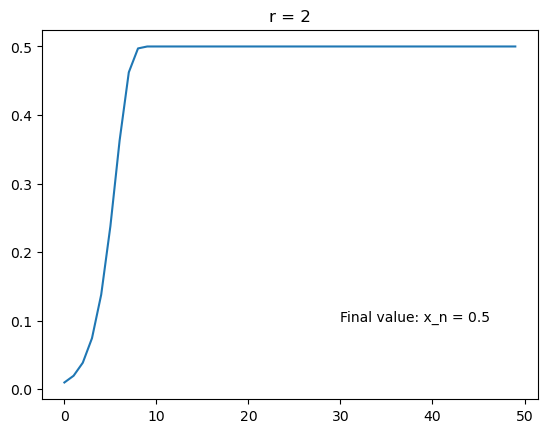
\includegraphics[scale=0.4]{r=2.png}
	\end{center}

\end{frame}	

\begin{frame}
	\frametitle{Logistic Equation} 

	What happens if we start at some small \( x_0 = 0.01 \), and 
	apply the rule \( x_n = f(x_{n - 1}) \), where 
	\( f(x) = rx(1 - x) \), with \( r = 3 \)? 

	\pause
	\begin{center}
		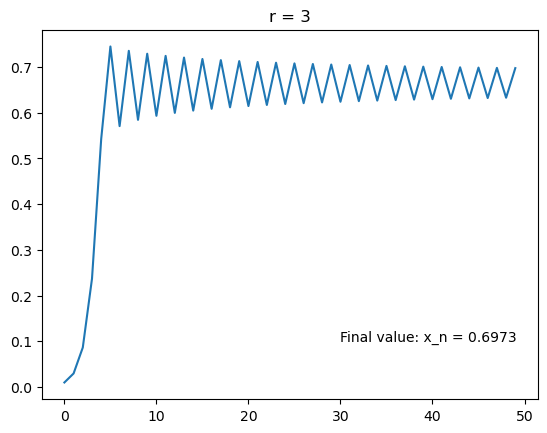
\includegraphics[scale=0.4]{r=3.png}
	\end{center}

	\begin{itemize}
		\item The first \( \sim \) 30 points do not oscillate 
			between the same two points, 
			and are called \textit{transients}
		\item Because they're not relevant to long-term behavior, 
			we will remove them in future plots. 
	\end{itemize}
\end{frame}

\begin{frame}
	\frametitle{Logistic Equation}

	What happens if we start at some small \( x_0 = 0.01 \), and 
	apply the rule \( x_n = f(x_{n - 1}) \), where 
	\( f(x) = rx(1 - x) \), with \( r = 3.5 \)? 
	
	\begin{center}
		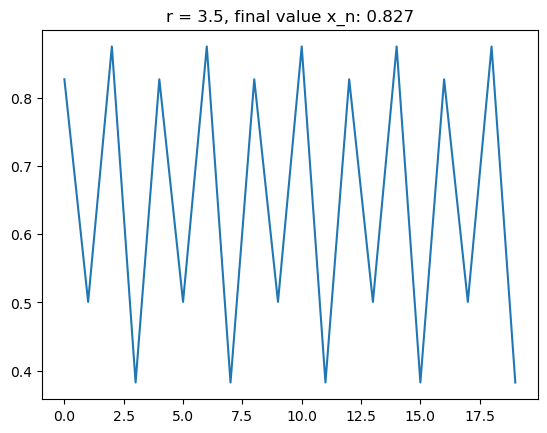
\includegraphics[scale=0.4]{r=3.5.png}
	\end{center}
	
	\pause
	\begin{itemize}
		\item Now \( x_n \) oscillates between 4 values \( \implies  \)
			4-cycle. 
	\end{itemize}
\end{frame}

\begin{frame}
	\frametitle{Logistic Equation}

	Now, let's try \( r = 3.66 \):

	\begin{center}
		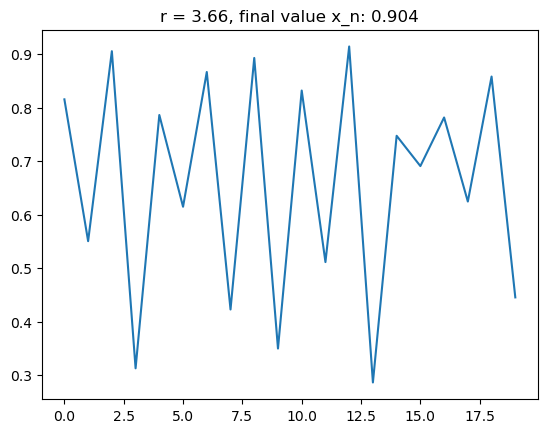
\includegraphics[scale=0.4]{r=3.66.png}
	\end{center}

	\pause 
	\begin{itemize}
		\item Is there any pattern here?
			\pause 
		\item Chaos!
	\end{itemize}
\end{frame}

\subsection{The Logistic Map}


\begin{frame}

	\frametitle{The Logistic Map}
	
	\begin{center}
		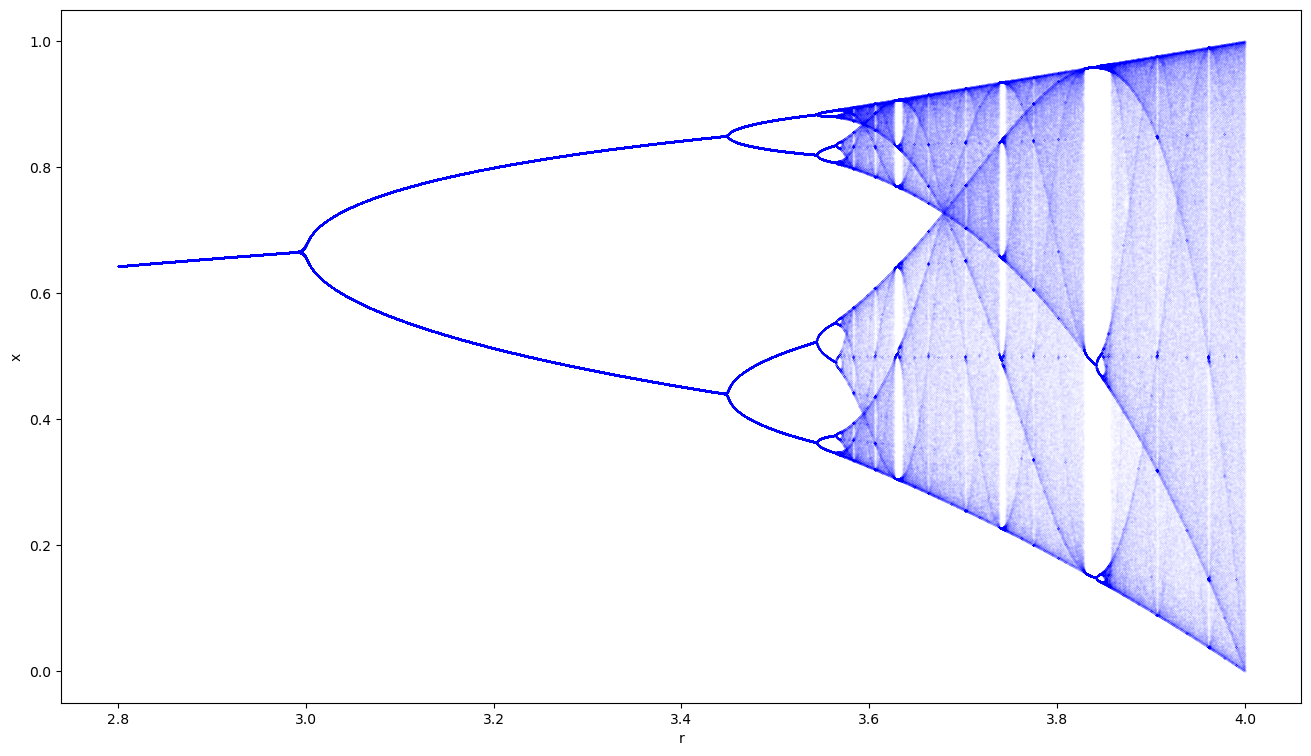
\includegraphics[width=\textwidth]{logistic-map.png}
	\end{center}
	\begin{itemize}
		\item Notice the period doublings!  
	\end{itemize}
\end{frame}

\begin{frame}
	\frametitle{Properties of the Logistic Map}

	\begin{itemize}
		\item First Feigenbaum constant
			\[
				\delta = \lim_{n \to \infty}\frac{d_{n + 1} - d_n}{d_n - d_{n - 1}}
				\approx 4.669\dots
			\]
			\( d_i \) is the difference between the \( i \)-th and the \( (i + 1)
			\)-th period doubling.
			\pause 
		\item Second Feigenbaum constant:
			\[
				\alpha = \frac{a_n}{a_{n + 1}} \approx 2.502\dots
			\]
			\( a_i \) is the width of the forks 
		\item Not much is known about either of these two numbers -- it is unknown if
			either of these are even irrational! 
		\item They are both universal constants: any chaotia equation of the form \(
			x_{n + 1} = \omega f(x_n) \) will have \( \alpha, \delta \) equal these
			values. 
	\end{itemize}
\end{frame}

\section{LabVIEW Simulations}

\subsection{Cobweb.VI}
\begin{frame}
	\frametitle{Cobweb.VI}

	\begin{itemize}
		\item Another way to visualize the progression of \( x_n \) as a function of
			\( n \). 
		\item From a sequence of values \( (m_0, \dots, m_n) \), we interleave the
			array with itself to get \( (m_0, m_0, \dots, m_n, m_n) \), then:
			\begin{itemize}
				\item \texttt{x\_values}: \( x_i = \{m_0, m_0, \dots, m_{n - 1}, m_{n
					- 1}\} \) 
				\item \texttt{y\_values}: \( y_i = \{0, m_1, m_1, \dots, m_{n - 1},
					m_n \}\)
			\end{itemize}
		\item Interleaving the \texttt{x\_values} with \texttt{y\_values}, we get the
			set of coordinates:
			\[
				(x_i, y_i) = \{(x_0, 0), (m_0, m_1), \dots, (m_{n - 1}, m_{n - 1}),
				(m_{n -1}, m_n)\}
			\]
	\end{itemize}
\end{frame}

\begin{frame}
	\begin{center}
		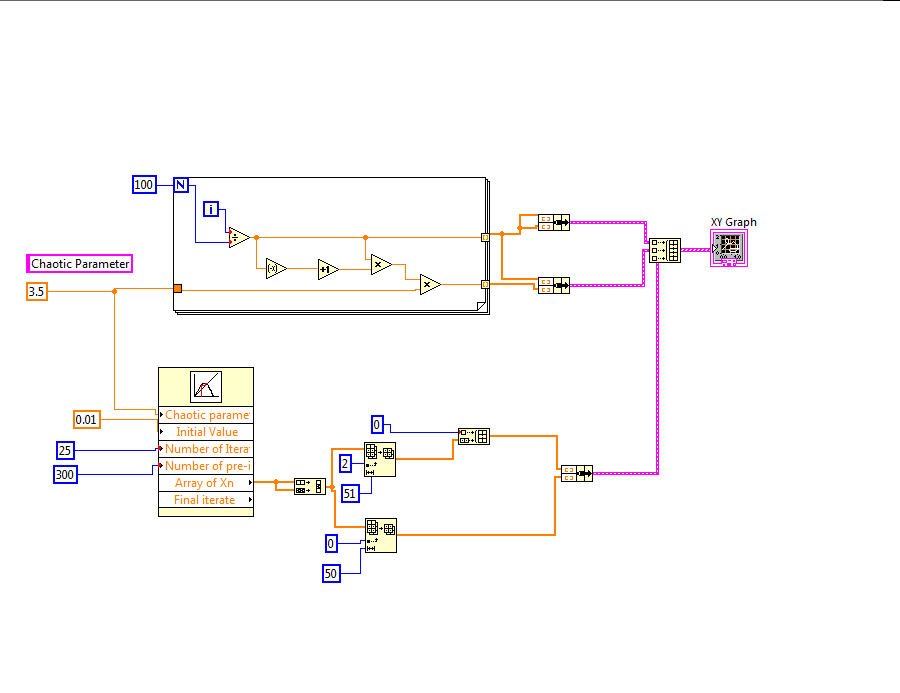
\includegraphics[scale=0.4]{images/cobweb_block}
	\end{center}
	% Maybe fix the line here
\end{frame}

\begin{frame}

	\frametitle{Visualization}

	\begin{center}
		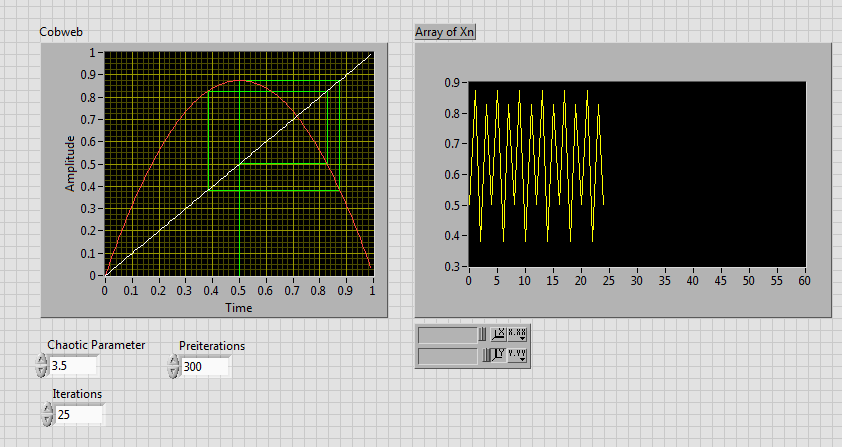
\includegraphics[scale=0.4]{images/cobweb_r_3.5_good.PNG}
	\end{center}
\end{frame}


\subsection{Lyapunov Exponent}

\begin{frame}

\frametitle{Lyapunov Exponent}
	\begin{itemize}
		\item \textbf{Sensitive Dependence on Initial Conditions:}    
			Trajectories which start off with an infinitesimal deviation 
			diverge exponentially quickly.  
		\item Suppose you have two initial conditions, \( x_0 \) and \( x_0 +
			\delta_0 \) where \( \delta_0 > 0 \) is the initial separation, and is very small. 
		\item Let \( \delta_n \) be the separation after \( n \) iterations. The
			Lyapunov exponent is defined as the value of \( \lambda \) such that 
			\( |\delta_n| = |\delta_0| e^{n \lambda} \). If \( \lambda > 0 \), then
			the trajectory is chaotic.
			\[
				\lambda = \lim_{n \to \infty}\frac{1}{n} \sum_{i = 0}^{n - 1} \ln |f'(x_i)|
			\]
		\item This formula comes from a linear approximation of the effect of \(
			\delta_{i+1} \) from \( \delta_{i} \) via linearization, hence the
			cumulative effect is a product, which decomposes to a sum over
			logarithms. 
	\end{itemize}
\end{frame}

\begin{frame}
	\frametitle{Procedure}
	\begin{itemize}
		\item For a fixed value of \( r \), allow the transients to die out, then
			compute a large number of iterates (10000).   
		\item Compute \( \ln |f(x_i)| = \ln |r - 2rx_n| \), and add all of them
			together. 
		\item Divide the final result by 10000 to get \( \lambda \).  
	\end{itemize}
\end{frame}

\begin{frame}
	\frametitle{LabVIEW Circuit}

	\begin{center}
		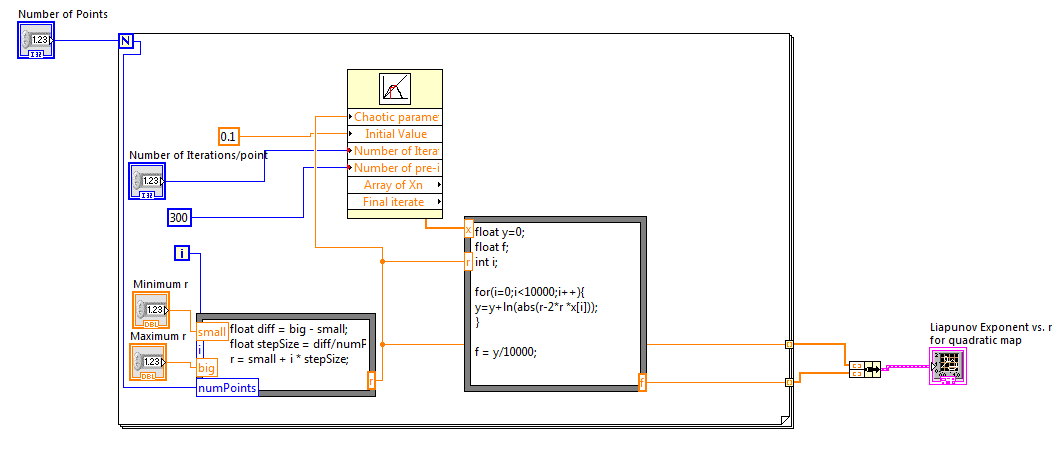
\includegraphics[scale=0.35]{images/LiapunovBlockDiagram}
	\end{center}
\end{frame}

\begin{frame}
	\frametitle{\( r = 3 \) to \( r = 4 \)}

	\begin{center}
		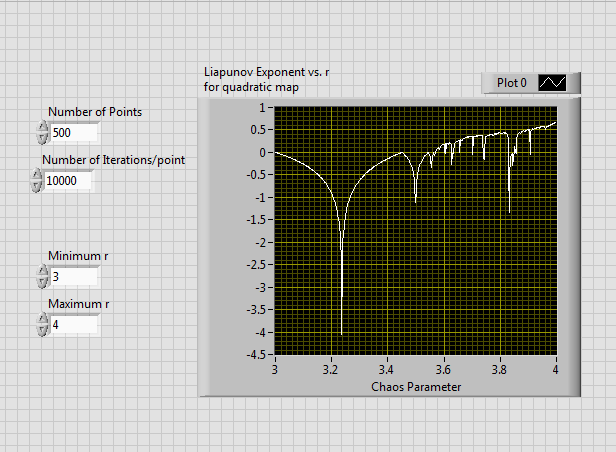
\includegraphics[scale=0.5]{images/liapunov_3_4.PNG}
	\end{center}
	\begin{itemize}
		\item Notice the increase from negative to positive at around 3.57 -- an
			indicator of chaos.   
	\end{itemize}
\end{frame}

\begin{frame}
	\frametitle{\( r = 3.55 \) to \( r = 3.59 \)}

	\begin{center}
		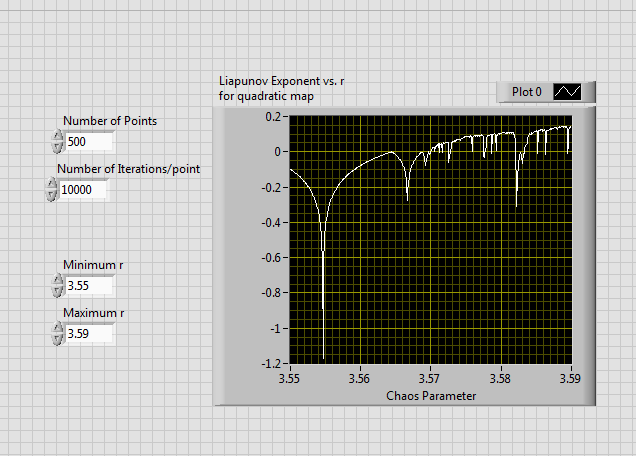
\includegraphics[scale=0.5]{images/liapunov_3.55_3.59}
	\end{center}
	\begin{itemize}
		\item Note that each spike should be
			infinitely deep, but are not due to numerical imprecision.  
	\end{itemize}
\end{frame}

\subsection{NLSim.VI}

\begin{frame}
	\frametitle{Return Map}
	\begin{itemize}
		\item Very similar to the Cobweb.VI, we plot \( (x_n, x_{n + 1}) \) on a 2D
			plane.   
		\item The \textbf{embedding dimension} is the dimension of phase space we choose to
			use. For a dimension 2, we only plot \( (x_n, x_{n + 1}) \). 
		\item For \( d =3 \), we would plot \( (x_n, x_{n + 1}, x_{n + 2}) \) in 3D. 
		\item Due to its qualitative nature, there is no real benefit to plot in
			higher dimensions for visual diagrams.   
	\end{itemize}
\end{frame}


\begin{frame}
	\frametitle{Short Aside: Fourier Series}
	\begin{itemize}
		\item A procedure that allows us to decompose any given signal into a set of
			sinusoids. In our case, because we are sampling a discrete set of points
			\( x_n \), then we need the Discrete Fourier Transform, generating a set
			of points:
			\[
				X_k = \sum_{n = 0}^{N - 1}x_n e^{- \frac{2\pi i kn}{N}}
			\]
			Here, \( N \) refers to the number of points. 
		\item Conceptually, it allows us to transform a signal in time into a signal
			in frequency. 
		\item For a sine wave, because it's a pure frequency, we expect the frequency
			domain plot to be a spike exactly at the frequency of the input wave.
	\end{itemize}
\end{frame}
\begin{frame}
	\frametitle{NLSim.VI}
	\begin{itemize}
		\item Input is a sine wave \( x(t) = \cos(\omega_1 t) \), we sample at \( f =
			f_s\) for \( N \) points. 
		\item We plot the sampled points vs. time, take the Fourier Transform, and
			also plot the \textit{return map}
			\begin{itemize}
				\item \textbf{Return map:} A plot of \( x_n \) vs. \( x_{n + 1} \) in
					2D space. 
			\end{itemize}
		\item Depending on the sampling rate, the sampled points may not give us back
			\( x(t) \), due to aliasing.
		\item Aliasing occurs when the highest frequency of the signal is larger than
			half the sampling frequency, or equivalently the sampling frequency is
			less than twice the bandwidth. 
			\begin{itemize}
				\item For a sine wave at frequency \( f \), its Fourier transform is
					two Delta functions at \( \pm f \), so \( \delta(f - f_0) +
					\delta(f + f_0) \). 
				\item The bandwidth is then \( 2f_0 \). 
			\end{itemize}
		\item The sampling rate also cannot be a multiple of the signal frequency in
			order for the return map to display properly. Otherwise, it will only
			show several points. 
	\end{itemize}
\end{frame}

% add the multisine wave

\begin{frame}
	\frametitle{LabVIEW Diagrams}

	\begin{center}
		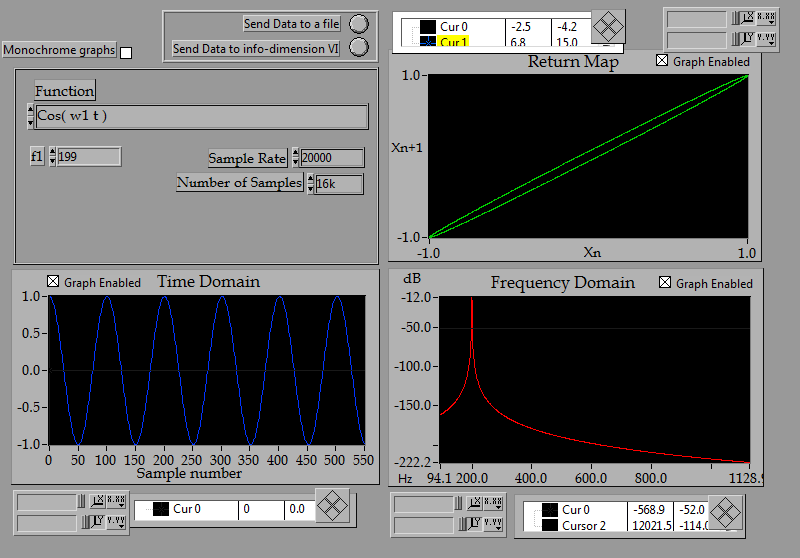
\includegraphics[scale=0.4]{images/nlsim_f_199_fs_20000_N_16k.PNG}
	\end{center}
	\begin{itemize}
		\item \( f_s = 20000 \) Hz, \( f = 199 \) Hz, so no aliasing. 
	\end{itemize}
\end{frame}

\begin{frame}
	\frametitle{LabVIEW Diagrams}

	\begin{center}
		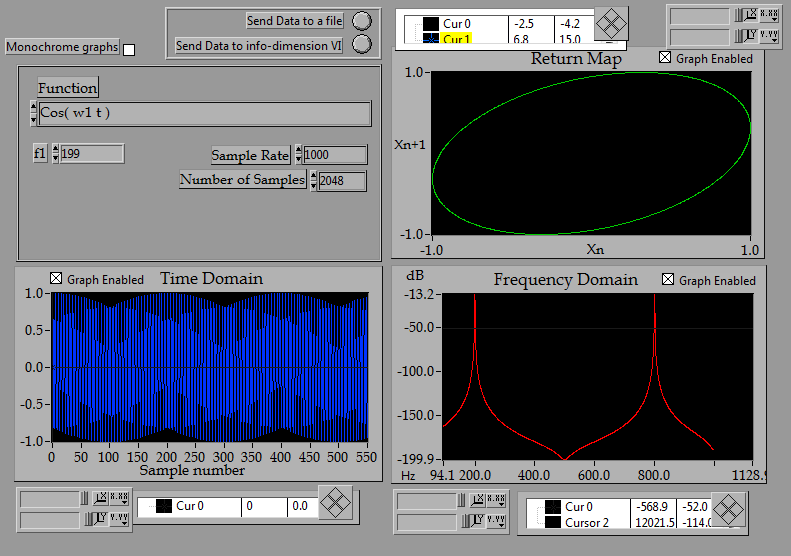
\includegraphics[scale=0.4]{images/nlsim_f_199_fs_1000.PNG}
	\end{center}
	\begin{itemize}
		\item \( f_s = 1000 \) Hz, \( f = 199 \) Hz, so we do have aliasing (as
			apparent in the frequency plot) 
	\end{itemize}
\end{frame}

\subsection{The Henon Map}
\begin{frame}
	\frametitle{Overview}
	\begin{itemize}
		\item The Henon map is another iterative system, except with a different
			equation. 
			\[
				\begin{cases}
					x_{n + 1} = 1 - ax_n^2 + y_n\\
					y_{n + 1} = bx_n
				\end{cases}
			\]
			There are two parameters \( a, b \) but \( a  \) is the only
			\textit{nonlinear} parameter. We will keep \( b \) fixed and vary \( a
			\).   
		\item We throw away the first 300 iterates, and compute 2000 iterates to
			generate the return map.  
	\end{itemize}
\end{frame}

\begin{frame}
	\frametitle{Return Map, \( a = 1.25 \)}

	\begin{center}
		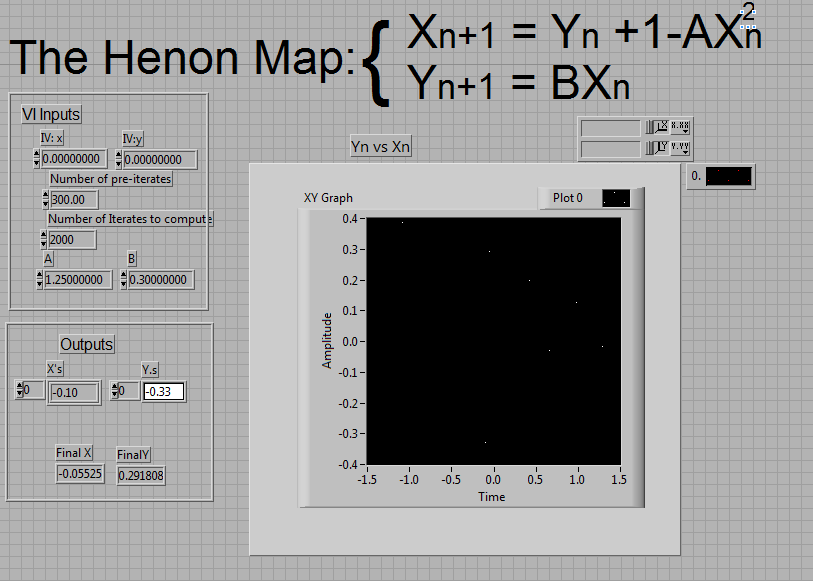
\includegraphics[scale=0.4]{images/HenonMap_1.25.PNG}
	\end{center}
	\begin{itemize}
		\item Notice that there are only 7 points, meaning that this motion is
			periodic. 
	\end{itemize}
\end{frame}

\begin{frame}
	\frametitle{Return Map, \( a = 1.4 \)}

	\begin{center}
		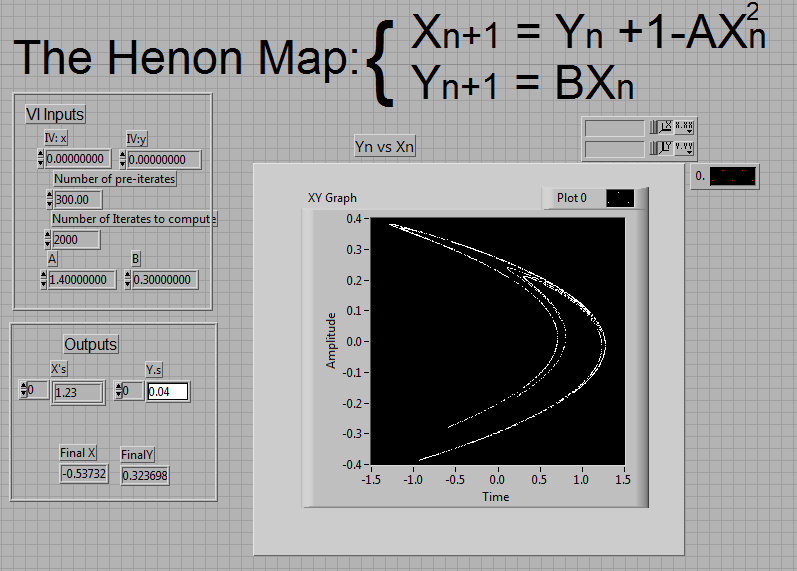
\includegraphics[scale=0.4]{images/HenonMap_1.4.PNG}	
	\end{center}
	\begin{itemize}
		\item The pattern doesn't seem to repeat this time, instead we see a
			\textit{strange attractor}.
	\end{itemize}
\end{frame}

\begin{frame}
	\frametitle{Bifurcation Diagram}
	\begin{itemize}
		\item Another way to visualize the Henon map is to plot the periodicity for
			multiple values of \( a \) simultaneously, giving a 2D bifurcation
			diagram. 

			\begin{center}
				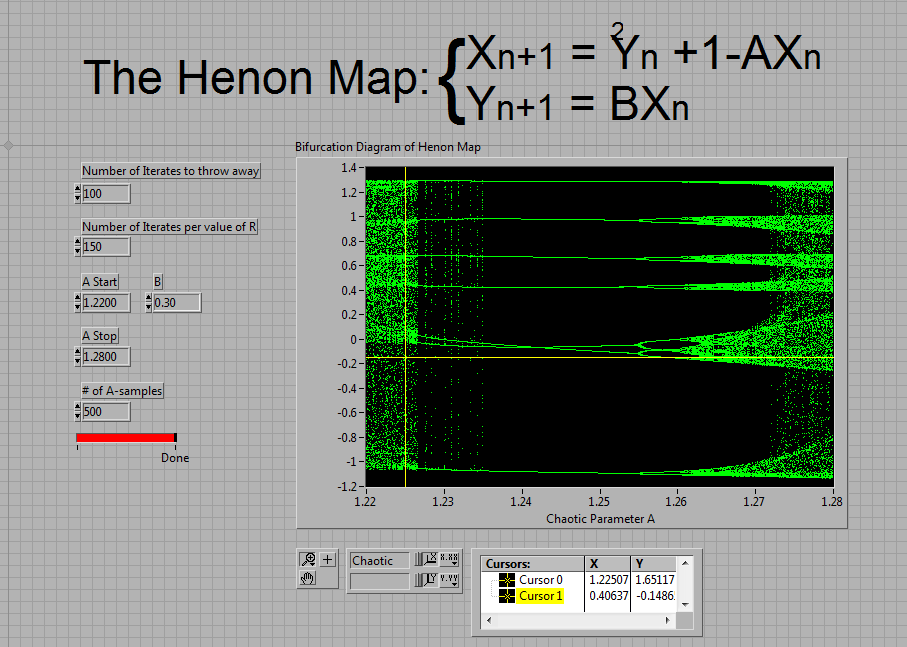
\includegraphics[scale=0.3]{images/HenonBifr.PNG}
			\end{center}
		\item Here we decided to zoom in on the region \( a = 1.22 \) to \( a = 1.28
			\), but in principle one can do this for any range. 
	\end{itemize}
\end{frame}

\begin{frame}
	\frametitle{3D Version} 

	\begin{center}
		\includegraphics[scale=0.05]{images/Henon_3D_Map.png}
	\end{center}	

\end{frame}
\section{Physical Circuitry}
\subsection{The PN Junction}
\begin{frame}
	\frametitle{Circuit Diagram}
	\begin{center}
		\begin{circuitikz}[scale=0.8]
			\draw (0, 0) to [sV, l = \( V(t) \)] (0, 4) to [L, l = \( L \)] (3, 4) to
			[full diode] (3, 0) to [R, l=\( R \)] (0, 0);
			\draw[dashed] (2.5, 3) rectangle (3.5, 1);
			\draw[dashed] (3.5, 3) -- (4, 4.5);
			\draw[dashed] (3.5, 1) -- (4, -0.5);
			\draw[dashed] (4, 4.5) rectangle (8.75, -0.5);
			\draw (4.5, 4) to (5, 4) to[capacitor, l=$C(V_d)$] (5, 0);
			\draw (5, 4) to (7, 4) to [american current source, l=$I_d(V_d)$] (7, 0)
			to (4.5, 0);
		\end{circuitikz}
		\begin{itemize}
			\item The nonlinear element is the diode, as it acts as an infinite
				resistor below \( V_d \) and as a current source above \( V_d \).    
		\end{itemize}
	\end{center}

\end{frame}

\begin{frame}
	\frametitle{Equations of Motion}

	The equations of motion for the PN junction circuit are provided to us: 
	\begin{align*}
		\dot I &= \frac{V_0 - RI - V_d}{L} \\ 
		\dot V_d &= \frac{I - I_d(V_d)}{C(V_d)} \\ 
		\dot \theta &= \omega
	\end{align*}
	These equations do not depend explicitly on time, and rather the future
	system only depends on the current state. \pause 
	Therefore, we if \( \vec p \)
	describes the current state in phase space, then we may write:
	\[
		\dot{\vec p} = F(\vec p)
	\]
	this is an iterative equation!
\end{frame}

\begin{frame}
	\frametitle{Bifurcation Diagram, \( V = 0 \) to \( V = 3.3 \)} 

	\begin{center}
		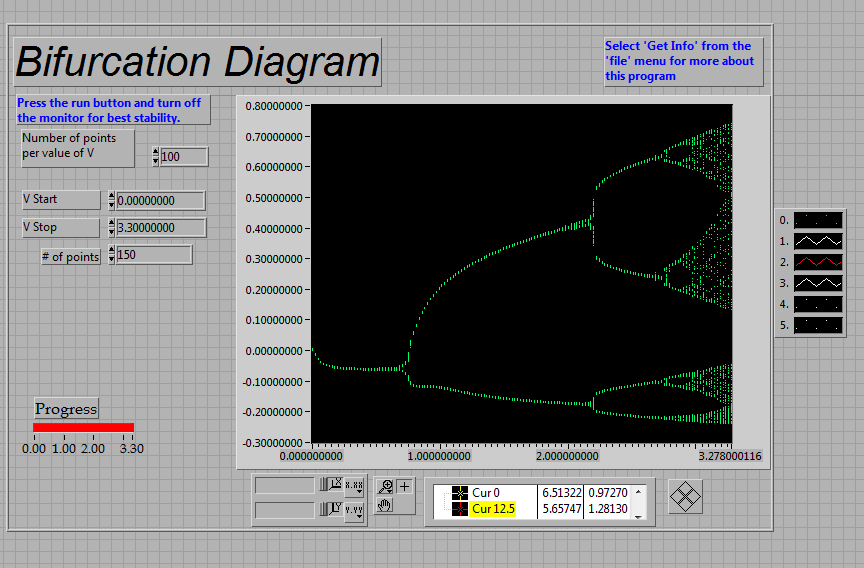
\includegraphics[scale=0.4]{images/NLDBifr_0_3.3.PNG}
	\end{center}
\end{frame}

\begin{frame}
	\frametitle{Bifurcation Diagram, \( V = 2.6 \) to \( V = 3.3 \)}
	\begin{center}
		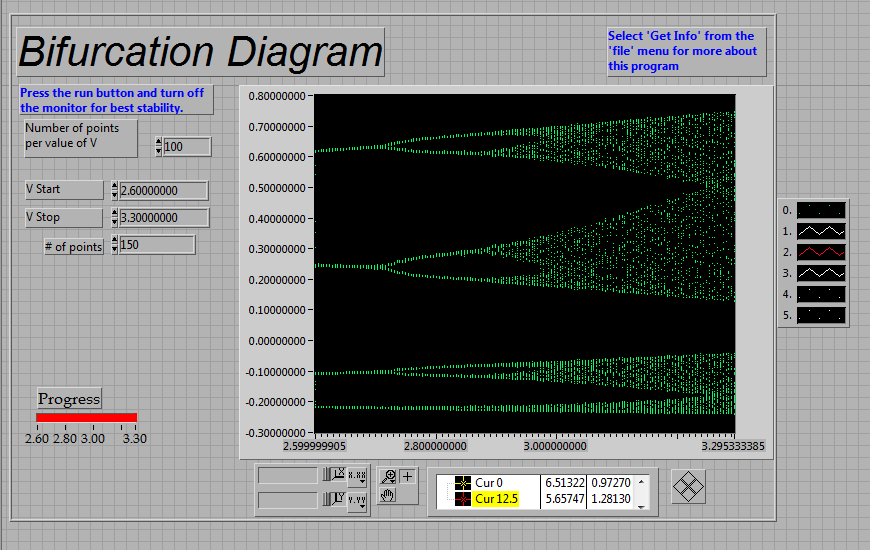
\includegraphics[scale=0.4]{images/NLDBifr_2.6_3.3.PNG}
	\end{center}

	% Talk about the bifurcation diagram and why it doesn't work very well 
	\begin{itemize}
		\item \( 1 \to 2 \) cycle: \( a =  0.786 \)
		\item \( 2 \to 4 \) cycle: \( a = 2.394 \)
		\item \( 4 \to 8 \) cycle: \( a = 3.092 \)
	\end{itemize}
\end{frame}

\begin{frame}
	\frametitle{Feigenbaum Ratio}
	\begin{itemize}
		\item With three values, there is only a single value of \( \delta \) we can
			calculate:
			\[
				\delta = \frac{2.394 - 0.786}{3.092 - 2.394} \approx 2.303
			\]
		\item This is a far cry from the expected \( \delta \approx 4.669 \), but
			remember that \( \delta  \) is a \textit{limit}, so we don't expect the
			first few \( \delta_n \) to match. 
		\item We could have gone further with higher precision, unfortunately we did
			not consider doing this during the lab.  
	\end{itemize}
\end{frame}

\subsection{Bouncing Ball}
\begin{frame}
	\frametitle{Bouncing Ball Circuit}
	\begin{itemize}
		\item Circuit simulates bouncing a ball on a table that is oscillating vertically
			according to a sine wave. 
		\item Actual circuitry is a black box and not provided to us :(  
	\end{itemize}
	\begin{center}
		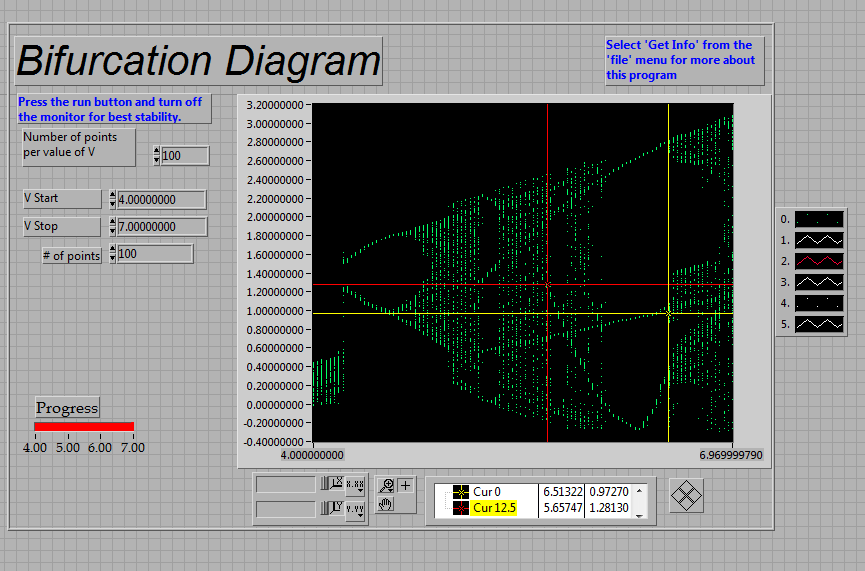
\includegraphics[scale=0.3]{images/BB_Bifr_4V-7V.PNG}
	\end{center}
	\begin{itemize}
		\item Unlike the PN Junction, there are no real indicators for period
			doubling. 
		\item Expected, since the motion of the ball is more complex and heavily
			depends on when the previous "bounce" occurred, so we cannot immediately
			write \( \dot{\vec p} = F(\vec p) \)
	\end{itemize}
\end{frame}

\subsection{Dimensionality}
\begin{frame}
	\frametitle{Box Dimension}
	\begin{itemize}
		\item How do we extend our intuitive understanding of dimension for fractals?
		\item Consider a square of width \( \epsilon \). Let \( N(\epsilon) \)
			be the number of \( \epsilon \)-squares required to cover the entire
			fractal. Then:
			\[
				d = \lim_{n \to \infty}\frac{\ln N(\epsilon)}{\ln(1 / \epsilon)}
			\]
		\item Conceptually, I think of this in the same way that the Gamma function
			\( \Gamma(z) \) extends our normal understanding of the factorial.
	\end{itemize}
\end{frame}

\begin{frame}
	\frametitle{Example}
	\begin{center}
		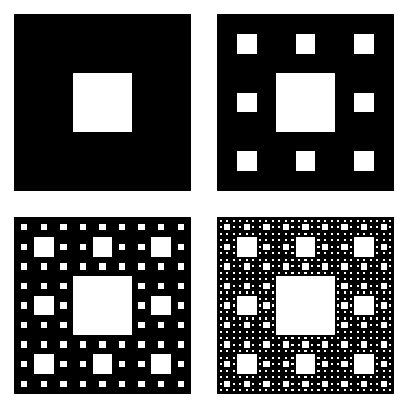
\includegraphics[scale=0.3]{images/sierpinski_carpet.png}
	\end{center}
	\begin{itemize}
		\item The first level is covered by 8 squares of length \( \frac{1}{3} \)
		\item The second level is covered by \( 8^2 = 64 \) squares of side length \(
			\frac{1}{3^2}\). 
		\item The \( n \)-th level is covered by \( 8^{n} \) squares of side length
			\( \frac{1}{3^{n}} \).
			\[
				d = \lim_{n \to \infty}\frac{\ln 8^{n}}{\ln (\frac{1}{3^{n}})} =
				\frac{\ln 8}{\ln 3} = 1.892\dots
			\]
	\end{itemize}
\end{frame}

\begin{frame}
	\frametitle{Information Dimension}
	\begin{itemize}
		\item Box dimension is nice when you can iteratively generate the fractal,
			and that the covering with squares is nice. How does one even define a
			minimal covering?       
		\item Information dimension is an alternative to this: take a point \( x \)
			in phase space, let \( N_x(\epsilon) \) be the number of points within an
			\( \epsilon \)-ball around \( x \). Conceptually, \( N_x(\epsilon) \),
			measures the number of points which are a distance \( \epsilon \) from
			\( x \).
		\item \( N_x(\epsilon) \propto \epsilon^{d}\), and taking the average over
			many points \( x \) we get the \textit{correlation dimension}
			\[
				C(\epsilon) \propto \epsilon^{d}
			\]
		\item \( C(\epsilon) \) is calculated using \texttt{CALCCORR.VI}, then we use
			Python to fit a slope to them. 
		\item In order to capture the maximum correlation, we want to use the highest
			embedding dimension possible, in our case we have \( n = 5 \). 
	\end{itemize}
\end{frame}

\begin{frame}
	\frametitle{Plot of \( C(\epsilon) \)}
	\begin{center}
		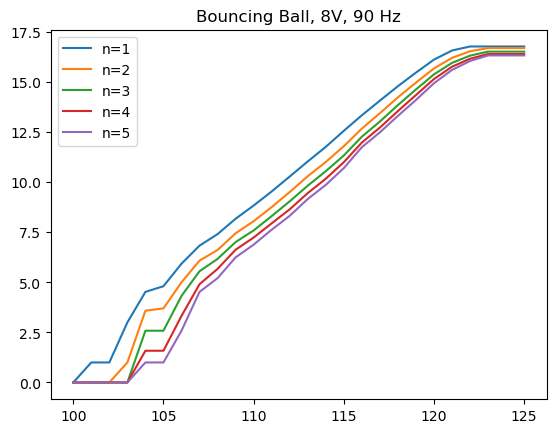
\includegraphics[scale=0.5]{images/corr_example.png}
	\end{center}
\end{frame}

\begin{frame}
	\frametitle{PN Junction}

	\begin{center}
		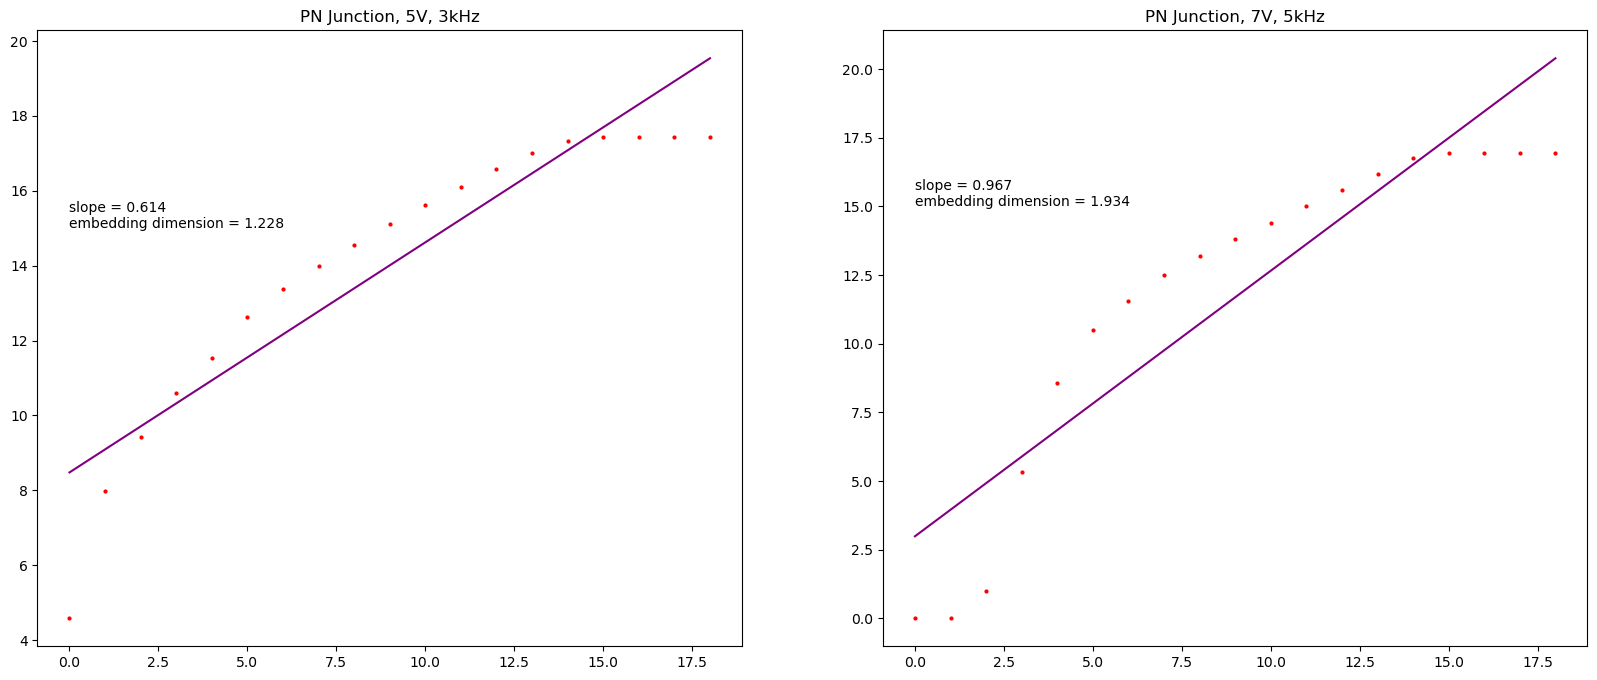
\includegraphics[scale=0.23]{images/PN_info_dimension.png}
	\end{center}
\end{frame}

\begin{frame}
	\frametitle{Bouncing Ball} 

	\begin{center}
		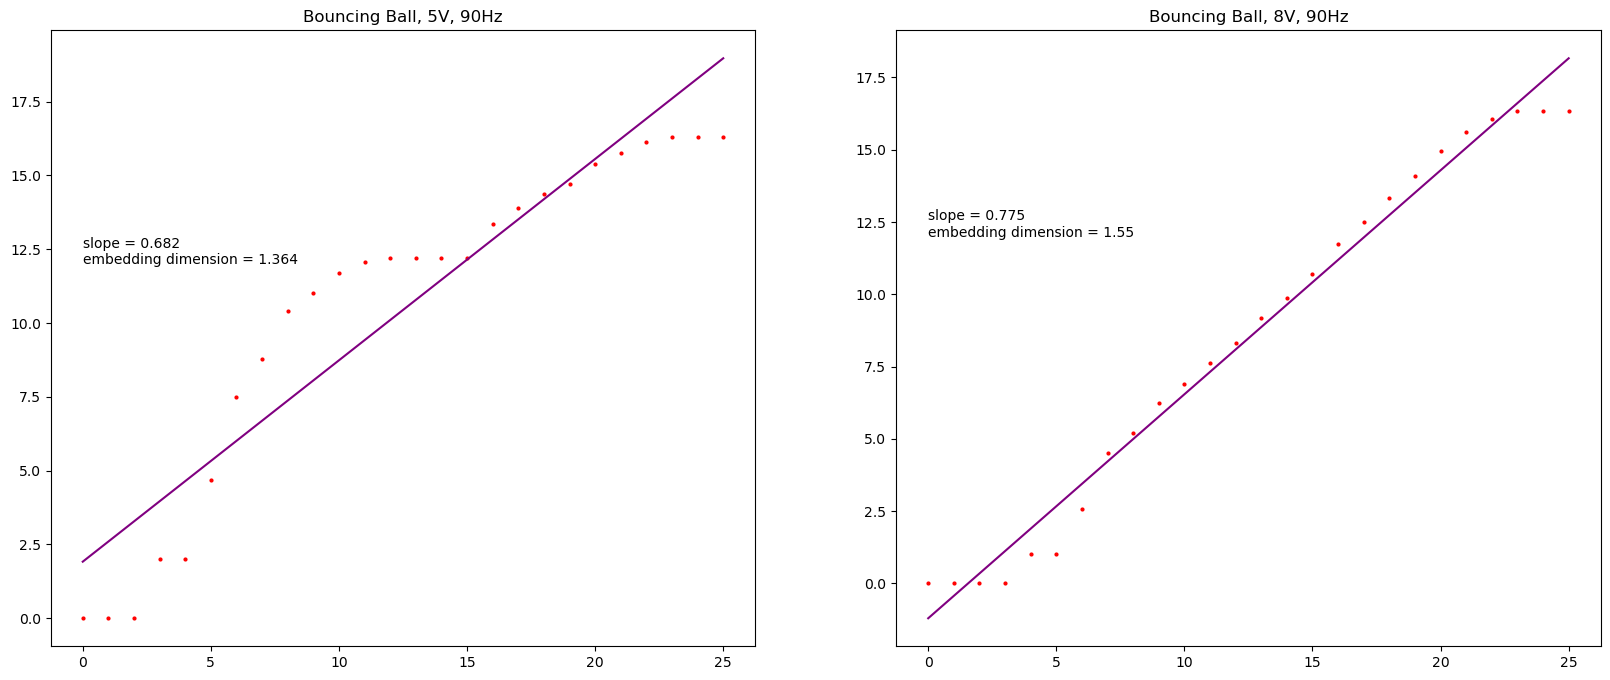
\includegraphics[scale=0.23]{images/BB_info_dimension.png}
	\end{center}

\end{frame}

\section{Conclusion}

\begin{frame}
	\frametitle{Summary}
	\begin{itemize}
		\item For systems that exhibit more chaotic features, the embedding dimension
			seems to be higher. 
			\begin{itemize}
				\item This makes sense, since chaotic systems by nature get
					arbitrarily close to a point \( x \) in phase space without being
					periodic. 
				\item For conservative systems, the information dimension should also
					be integral. 
			\end{itemize}
		\item The information dimension for the Bouncing ball is lower than that of
			the PN junction. 
		\item The PN Junction circuit is an example of an iterative chaotic system,
			so we get a bifurcation diagram very similar to that of the logistic map.    
		\item We didn't really go into possible error sources in this process since
			most of it was electronic and numerical, but the two main sources of
			error would be the circuit elements themselves and numerical imprecision
			of numerical operations in computers.
	\end{itemize}
\end{frame}

\begin{frame}
	\frametitle{Overall Thoughts on the Lab}
	\begin{itemize}
		\item This was a fun lab!
		\item We missed a couple things: like writing down whether the configurations
			we were using for information dimension were chaotic or not.
			\begin{itemize}
				\item The periodicity (or lack thereof) plays a large role 
					in information dimension.
			\end{itemize}
		\item Enjoyed playing around with a physical oscilloscope for the first time,
			in 111A we used Waveforms only. 
		\item LabVIEW was a pain at times. 
	\end{itemize}
\end{frame}

\begin{frame}{References}
	\fontsize{10pt}{12pt}\selectfont
	\nocite{*}
	\bibliographystyle{unsrt} 
	\bibliography{NLD}
\end{frame}
% include references
\end{document}
